\documentclass[handout]{beamer}\usepackage[]{graphicx}\usepackage[]{color}
%% maxwidth is the original width if it is less than linewidth
%% otherwise use linewidth (to make sure the graphics do not exceed the margin)
\makeatletter
\def\maxwidth{ %
  \ifdim\Gin@nat@width>\linewidth
    \linewidth
  \else
    \Gin@nat@width
  \fi
}
\makeatother

\definecolor{fgcolor}{rgb}{0.345, 0.345, 0.345}
\newcommand{\hlnum}[1]{\textcolor[rgb]{0.686,0.059,0.569}{#1}}%
\newcommand{\hlstr}[1]{\textcolor[rgb]{0.192,0.494,0.8}{#1}}%
\newcommand{\hlcom}[1]{\textcolor[rgb]{0.678,0.584,0.686}{\textit{#1}}}%
\newcommand{\hlopt}[1]{\textcolor[rgb]{0,0,0}{#1}}%
\newcommand{\hlstd}[1]{\textcolor[rgb]{0.345,0.345,0.345}{#1}}%
\newcommand{\hlkwa}[1]{\textcolor[rgb]{0.161,0.373,0.58}{\textbf{#1}}}%
\newcommand{\hlkwb}[1]{\textcolor[rgb]{0.69,0.353,0.396}{#1}}%
\newcommand{\hlkwc}[1]{\textcolor[rgb]{0.333,0.667,0.333}{#1}}%
\newcommand{\hlkwd}[1]{\textcolor[rgb]{0.737,0.353,0.396}{\textbf{#1}}}%
\let\hlipl\hlkwb

\usepackage{framed}
\makeatletter
\newenvironment{kframe}{%
 \def\at@end@of@kframe{}%
 \ifinner\ifhmode%
  \def\at@end@of@kframe{\end{minipage}}%
  \begin{minipage}{\columnwidth}%
 \fi\fi%
 \def\FrameCommand##1{\hskip\@totalleftmargin \hskip-\fboxsep
 \colorbox{shadecolor}{##1}\hskip-\fboxsep
     % There is no \\@totalrightmargin, so:
     \hskip-\linewidth \hskip-\@totalleftmargin \hskip\columnwidth}%
 \MakeFramed {\advance\hsize-\width
   \@totalleftmargin\z@ \linewidth\hsize
   \@setminipage}}%
 {\par\unskip\endMakeFramed%
 \at@end@of@kframe}
\makeatother

\definecolor{shadecolor}{rgb}{.97, .97, .97}
\definecolor{messagecolor}{rgb}{0, 0, 0}
\definecolor{warningcolor}{rgb}{1, 0, 1}
\definecolor{errorcolor}{rgb}{1, 0, 0}
\newenvironment{knitrout}{}{} % an empty environment to be redefined in TeX

\usepackage{alltt}

\usetheme{Madrid}
\usepackage{tikz}
\usepackage{underscore}
%\usepackage{lmodern}
%\usepackage[english]{babel}
\usepackage{enumerate}
%\usepackage{graphicx}
%\usepackage{array}
%\usepackage{multirow}
%\usepackage{multicol}
\beamertemplatenavigationsymbolsempty

%Bibliography 
\usepackage[backend=bibtex,style=bwl-FU]{biblatex}
\renewcommand*{\nameyeardelim}{\addcomma\addspace}
\usetikzlibrary{arrows,shapes}
\usefonttheme[onlymath]{serif}


\addbibresource{Literature.bib}


\title{Bayesian Analysis in R: brms vs rstanarm}
\author{Alice Milivinti\newline\url{a.lice.milivinti@gmail.com}}}
\date{12 april 2018}
\IfFileExists{upquote.sty}{\usepackage{upquote}}{}
\begin{document}




%%%%%%%%%%%%%%%%%%%%%%%%%%%%%%%%%%%%%%%%%%%%%%%%%%%%%%%%%%

\frame{\titlepage}

%%%%%%%%%%%%%%%%%%%%%%%%%%%%%%%%%%%%%%%%%%%%%%%%%%%%%%%%%%
\begin{frame}
\frametitle{Bayesians vs Frequentist}
\begin{figure}
\centering
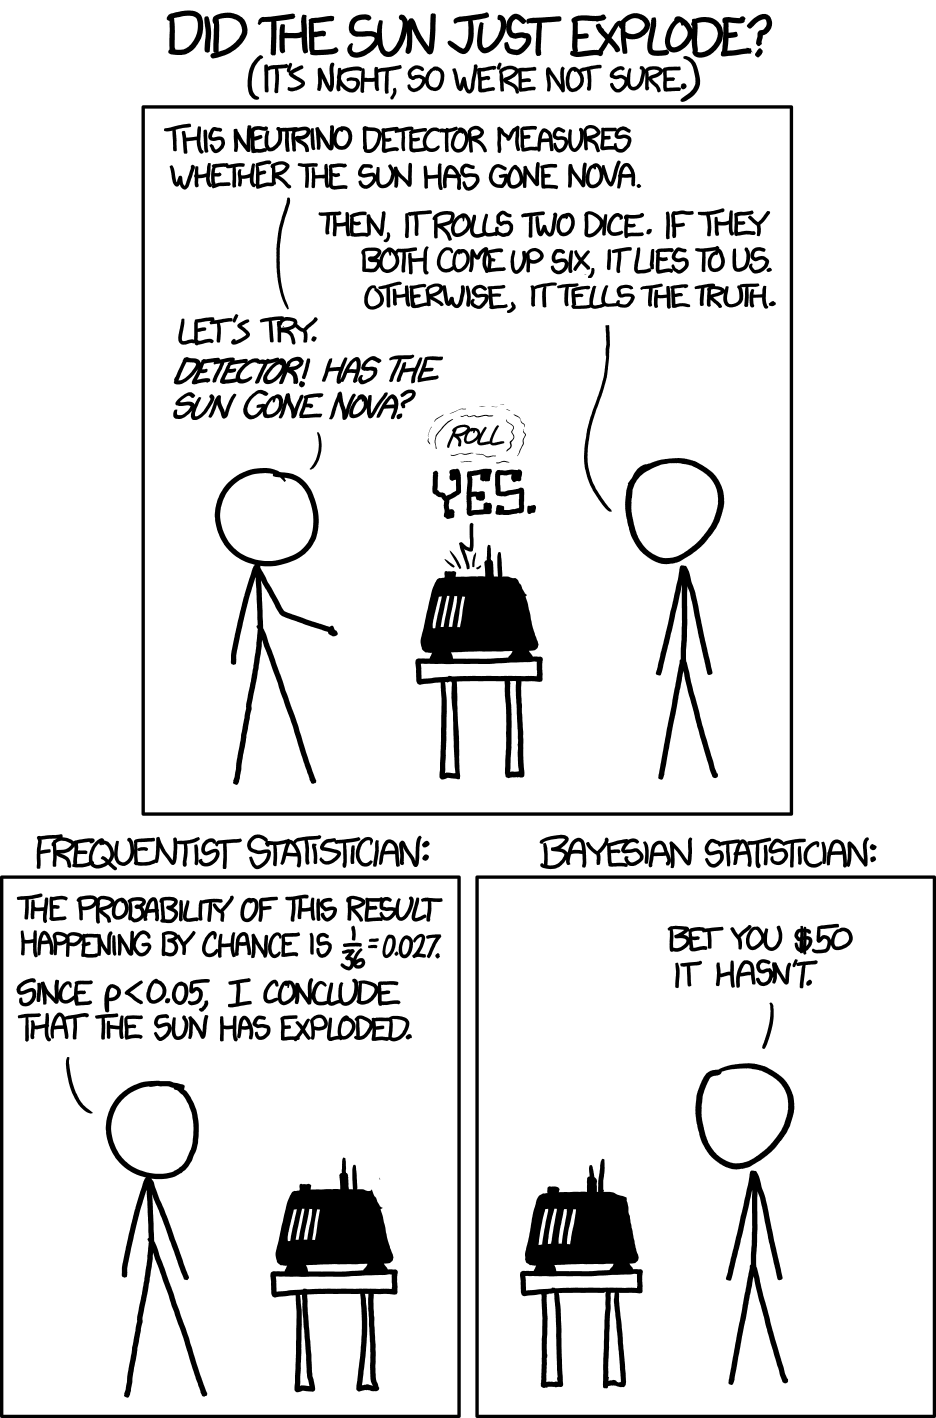
\includegraphics[scale=.3]{bayesians.png}
\end{figure}
\end{frame}

%%%%%%%%%%%%%%%%%%%%%%%%%%%%%%%%%%%%%%%%%%%%%%%%%%%%%%%%%%

\begin{frame}
\frametitle{Probability is...}
\pause
{\Large \textbf{Frequentists}} \\
\vskip 1cm
\pause
Fundamentally related to the frequencies of repeated events. 
\pause
\begin{align*}
\mathbf{Pr(A \mid B) \propto Pr(B \mid A) }
\end{align*}
%approximately proportional to...
$Pr(A \mid B)$: Posterior; \\
$Pr(B \mid A)$: Likelihood = Data Knowledge. \\
\pause
Given the observed data, what is the best estimate of the true value?

\end{frame}

%%%%%%%%%%%%%%%%%%%%%%%%%%%%%%%%%%%%%%%%%%%%%%%%%%%%%%%%%%

\begin{frame}
\frametitle{Maximum Likelihood}
\pause
Model: each observation $A_i$ drawn from a Gaussian of width $e_{i}$
% Gaussian centered at the observed value and with width given by the error
\begin{align*}
P(B_{i} \mid A_{true}) =  \frac{1}{\sqrt{2 \pi e_{i}^2}} \exp \left[ -\frac{(A_{i} - A_{true})^2}{2 e_{i}} \right]
\end{align*}




\begin{knitrout}
\definecolor{shadecolor}{rgb}{0.969, 0.969, 0.969}\color{fgcolor}
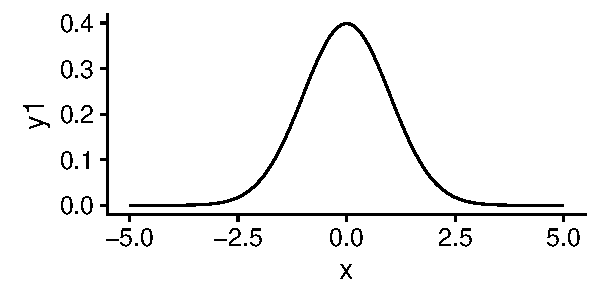
\includegraphics[width=\maxwidth]{figure/unnamed-chunk-1-1} 

\end{knitrout}

\end{frame}

%%%%%%%%%%%%%%%%%%%%%%%%%%%%%%%%%%%%%%%%%%%%%%%%%%%%%%%%%%
\begin{frame}
\frametitle{Buldind the Maximum Likelihood}
\begin{align*}
\mathcal{L}(B \mid A_{true}) =  \prod_{i=1}^{N} P(B_{i} \mid A_{true})
\end{align*}

\begin{knitrout}
\definecolor{shadecolor}{rgb}{0.969, 0.969, 0.969}\color{fgcolor}
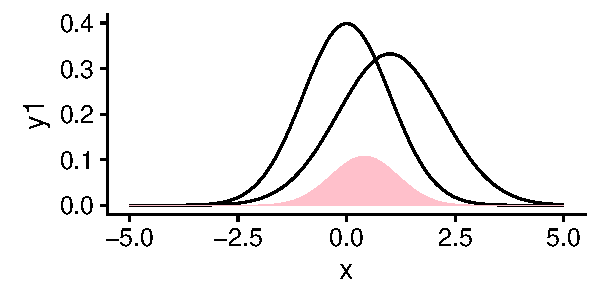
\includegraphics[width=\maxwidth]{figure/unnamed-chunk-2-1} 

\end{knitrout}

%What happens for each single measurement.
\end{frame}

%%%%%%%%%%%%%%%%%%%%%%%%%%%%%%%%%%%%%%%%%%%%%%%%%%%%%%%%%%
\begin{frame}
\frametitle{Buldind the Maximum Likelihood}
\begin{align*}
\mathcal{L}(B \mid A_{true}) =  \prod_{i=1}^{N} P(B_{i} \mid A_{true})
\end{align*}


\begin{knitrout}
\definecolor{shadecolor}{rgb}{0.969, 0.969, 0.969}\color{fgcolor}
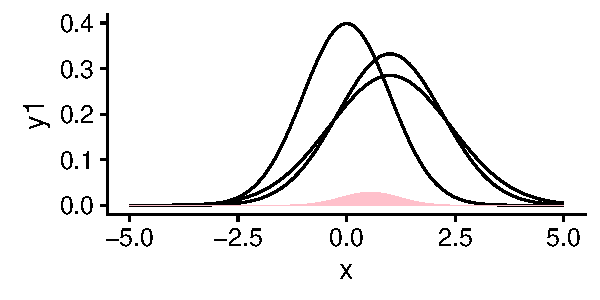
\includegraphics[width=\maxwidth]{figure/unnamed-chunk-3-1} 

\end{knitrout}


\end{frame}

%%%%%%%%%%%%%%%%%%%%%%%%%%%%%%%%%%%%%%%%%%%%%%%%%%%%%%%%%%
\begin{frame}
\frametitle{Buldind the Maximum Likelihood}
\begin{align*}
\mathcal{L}(B \mid A_{true}) =  \prod_{i=1}^{N} P(B_{i} \mid A_{true})
\end{align*}

\begin{knitrout}
\definecolor{shadecolor}{rgb}{0.969, 0.969, 0.969}\color{fgcolor}
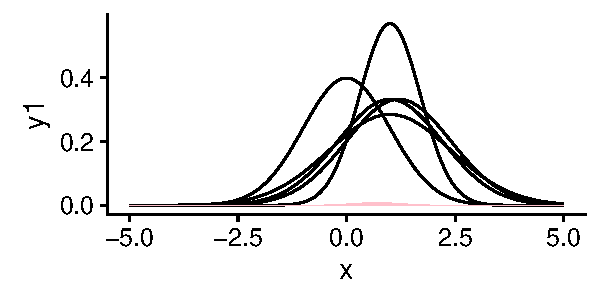
\includegraphics[width=\maxwidth]{figure/unnamed-chunk-4-1} 

\end{knitrout}


\end{frame}

%%%%%%%%%%%%%%%%%%%%%%%%%%%%%%%%%%%%%%%%%%%%%%%%%%%%%%%%%%

\begin{frame}
\frametitle{Probability is...}
\pause
{\Large \textbf{Bayesian}} \\
\vskip 1cm
\pause
Fundamentally related to {\color{green} OUR OWN} certainty or uncertainty of events.
\pause
\begin{align*}
\mathbf{Pr(A \mid B) \propto Pr(B \mid A) {\color{green} Pr(A)} }
\end{align*}
$Pr(A \mid B)$: Posterior; \\
$Pr(B \mid A)$: Likelihood = Data Knowledge. \\
${\color{green} Pr(A)}$: Prior = Our Knowledge.

\end{frame}

%%%%%%%%%%%%%%%%%%%%%%%%%%%%%%%%%%%%%%%%%%%%%%%%%%%%%%%%%%
\begin{frame}
\frametitle{Prior, Likeloihood and Posterior}
\pause
\begin{align*}
\mathbf{{\color{blue} Pr(A \mid B)} \propto \color{red} {Pr(B \mid A) } {\color{green} Pr(A)} }
\end{align*}
\pause


\begin{knitrout}
\definecolor{shadecolor}{rgb}{0.969, 0.969, 0.969}\color{fgcolor}
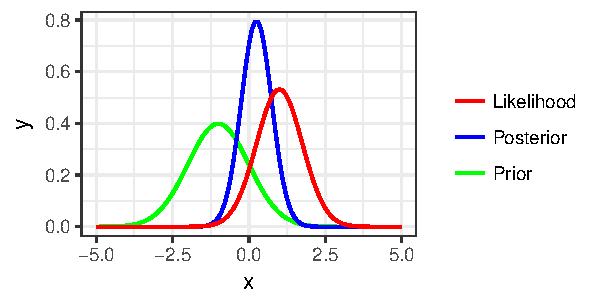
\includegraphics[width=\maxwidth]{figure/bayes-1} 

\end{knitrout}

\end{frame}

%%%%%%%%%%%%%%%%%%%%%%%%%%%%%%%%%%%%%%%%%%%%%%%%%%%%%%%%%%

\begin{frame}
\frametitle{A word on the priors...}
\pause
Priors can be: informative, weakly informative or uninformative. \\
\pause
A Bayesian analysis which uses an uninformative prior, such as
\pause
\begin{align*}
\mathcal{U} \left( -\infty, +\infty \right)
\end{align*}
\pause
will give the same result as a frequentist analysis.

\begin{knitrout}
\definecolor{shadecolor}{rgb}{0.969, 0.969, 0.969}\color{fgcolor}
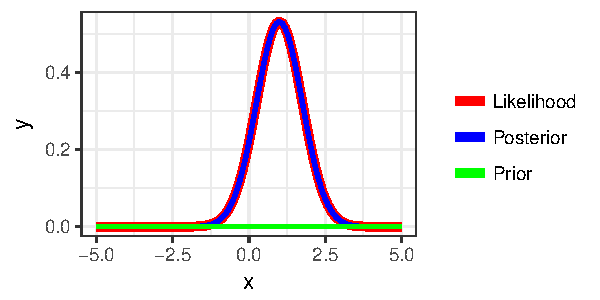
\includegraphics[width=\maxwidth]{figure/uniform-1} 

\end{knitrout}

\end{frame}

%%%%%%%%%%%%%%%%%%%%%%%%%%%%%%%%%%%%%%%%%%%%%%%%%%%%%%%%%%

\begin{frame}
\frametitle{Sample the Posterior}

So far we have investigated how to use Bayesian techniques to determine posterior probability distribution for a set of parameters in light of some data. \\
\pause
However, our parameter set may be highly-dimensional, and we may only be interested in a sub-set of (marginalized) parameters. \\
\pause
\textbf{Markov Chain Monte Carlo (MCMC) is an efficient approach to this problem.}

\end{frame}

%%%%%%%%%%%%%%%%%%%%%%%%%%%%%%%%%%%%%%%%%%%%%%%%%%%%%%%%%%

\begin{frame}
\frametitle{Markov Chain Monte Carlo}

Straight-forward Monte Carlo integration suffers from some problems...(especially if your posterior probability is peaked in a small volume of your parameter space).\\
\pause
Need for a method to throw down more points into the volume in regions of interest, and not waste points where the integrand is negligible. \\
\pause
We can use a Markov Chain to “walk” through the parameter space, vagabonding in regions of high significance, and avoiding everywhere else.
\pause
\textbf{MCMC Algorithms: ex. Metropolis-Hasting, Gibbs, etc.}
\end{frame}

%%%%%%%%%%%%%%%%%%%%%%%%%%%%%%%%%%%%%%%%%%%%%%%%%%%%%%%%%%

\begin{frame}
\frametitle{Frequestist Approach}

Frequentism is a probabilistic statement about a recipe for generating confidence intervals given a fixed model parameter
\pause
\begin{figure}
\centering

\includegraphics[scale=.25]{Frequentist2.png}
\end{figure}
{\tiny \textit{Credits:} \textcite{vanderplas2014}}
\end{frame}


%%%%%%%%%%%%%%%%%%%%%%%%%%%%%%%%%%%%%%%%%%%%%%%%%%%%%%%%%%
\begin{frame}
\frametitle{Bayesian Approach}

\pause
Bayesianism is aprobabilisitic statement about model parameters given a fixed credible region
\pause

\begin{figure}
\centering
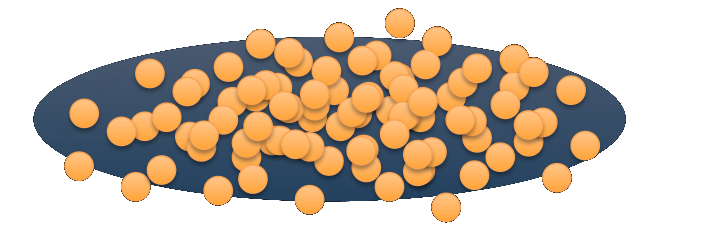
\includegraphics[scale=.25]{Bayesian2.png}
\end{figure}
{\tiny \textit{Credits:} \textcite{vanderplas2014}}


\end{frame}

%%%%%%%%%%%%%%%%%%%%%%%%%%%%%%%%%%%%%%%%%%%%%%%%%%%%%%%%%%

\begin{frame}
\frametitle{Please Remember This}
\pause
A frequentist 95\% confidence interval is NOT 95\% likely to contain the true value! \\ 
\pause
\vskip 1cm
This very common mistake is a Bayesian interpretation of a frequentist construct. \\

\end{frame}

%%%%%%%%%%%%%%%%%%%%%%%%%%%%%%%%%%%%%%%%%%%%%%%%%%%%%%%%%%

\begin{frame}
\frametitle{Take Home Message}

\textbf{Frequentists}
A 95\% of such Confidence Intervals in repeated experiments will contain the true value! \\
\vskip 1cm
\pause
\textbf{Bayesians}
A 95\% Credible Region is 95\% likely to contain the true value! \\
\end{frame}



%%%%%%%%%%%%%%%%%%%%%%%%%%%%%%%%%%%%%%%%%%%%%%%%%%%%%%%%%%

\begin{frame}
\frametitle{STAN}
\pause
Stan language \autocite{stan2015} which makes use of the Hamiltonian Monte-Carlo Sampler \autocite{neal2011mcmc} of Hybrid Monte-Carlo Sampler (HMC) \autocite{duane1987hybrid} and its extension No-U-Turn Sampler (NUTS) \autocite{hoffman2014no}. \\
\vskip .3cm
\pause

\begin{itemize}
\item Much higher effective sample size per iteration for complex posteriors.
\pause
\item  Overall, much higher number of effective samples per second.
\pause
\item Does not require any special behaviour for conjugate priors, which much impact the priors' choice \autocite{hoffman2014no}.
\end{itemize}

%Gibbs need conjugate priors

\end{frame}

%%%%%%%%%%%%%%%%%%%%%%%%%%%%%%%%%%%%%%%%%%%%%%%%%%%%%%%%%%

\begin{frame}
\frametitle{STAN \& R}
\pause
\begin{itemize}
\item \texttt{rstan}: R Interface to Stan C++ library for Bayesian estimation. Upload your stan code and run it through R. %then analyse results using dependencies
\vskip 1cm
\pause
\item \texttt{rstanarm} \& \texttt{brms}:  Estimate previously compiled regression models using \texttt{rstan}. Users specify models via the R syntax with a formula and data.frame plus some additional arguments for priors.  

\end{itemize}

\end{frame}
 
 
%%%%%%%%%%%%%%%%%%%%%%%%%%%%%%%%%%%%%%%%%%%%%%%%%%%%%%%%%%

\begin{frame}
\frametitle{\texttt{rstanarm} \& \texttt{brms}}

\begin{columns}[onlytextwidth,t]
\begin{column}{0.48\textwidth}
\texttt{rstanarm} \\
\begin{itemize}
\item manual's pages: 121
\item topics documented: 47
\item authors \& contributors: 17, Jonah Gabry, Imad Ali, Sam Brilleman, Jacqueline Buros Novik, AstraZeneca, Trustees of Columbia University, Simon Wood, R Core Deveopment Team, Douglas Bates, Martin Maechler, Ben Bolker, Steve Walker, Brian Ripley, William Venables, Ben Goodrich
\end{itemize}
\end{column}
\begin{column}{0.48\textwidth}  
\texttt{brms} \\
\begin{itemize}
\item manual's pages: 154
\item topics documented: 144 (so detailed!)
\item author: 1, Paul-Christian B\"{u}rkner \\
%He is ridiculously responsive in adding functions or helping with any problem
\end{itemize}
\end{column}
\end{columns}

\end{frame}

%%%%%%%%%%%%%%%%%%%%%%%%%%%%%%%%%%%%%%%%%%%%%%%%%%%%%%%% 

\begin{frame}[fragile]
\frametitle{Syntax Comparison with mtcars}
With default weakly informative priors: \\
\texttt{rstanarm}: \\

\begin{knitrout}
\definecolor{shadecolor}{rgb}{0.969, 0.969, 0.969}\color{fgcolor}\begin{kframe}
\begin{alltt}
\hlkwd{stan_glm}\hlstd{(}\hlkwc{formula} \hlstd{= mpg} \hlopt{~} \hlstd{wt} \hlopt{+} \hlstd{am} \hlopt{+} \hlstd{cyl,} \hlkwc{data} \hlstd{= mtcars,}
         \hlkwc{prior} \hlstd{=} \hlkwa{NULL}\hlstd{,} \hlkwc{family} \hlstd{=} \hlkwd{gaussian}\hlstd{(),} \hlkwc{chains} \hlstd{=} \hlnum{4}\hlstd{,}
         \hlkwc{iter} \hlstd{=} \hlnum{2000}\hlstd{,} \hlkwc{warmup} \hlstd{=} \hlnum{1000}\hlstd{)}
\end{alltt}
\end{kframe}
\end{knitrout}

\texttt{brms}: \\

\begin{knitrout}
\definecolor{shadecolor}{rgb}{0.969, 0.969, 0.969}\color{fgcolor}\begin{kframe}
\begin{alltt}
\hlkwd{brm}\hlstd{(}\hlkwc{formula} \hlstd{= mpg} \hlopt{~} \hlstd{wt} \hlopt{+} \hlstd{am} \hlopt{+} \hlstd{cyl,} \hlkwc{data} \hlstd{= mtcars,}
    \hlkwc{prior} \hlstd{=} \hlkwa{NULL}\hlstd{,} \hlkwc{family}  \hlstd{=} \hlstr{"gaussian"}\hlstd{,} \hlkwc{chains} \hlstd{=} \hlnum{4}\hlstd{,}
    \hlkwc{iter} \hlstd{=} \hlnum{2000}\hlstd{,} \hlkwc{warmup} \hlstd{=} \hlnum{1000}\hlstd{)}
\end{alltt}
\end{kframe}
\end{knitrout}


\end{frame}

%%%%%%%%%%%%%%%%%%%%%%%%%%%%%%%%%%%%%%%%%%%%%%%%%%%%%%%% 

\begin{frame}
\frametitle{system.time() and Marvok Chains}

\begin{columns}[onlytextwidth,t]
\begin{column}{0.48\textwidth}
\texttt{rstanarm}\\
system.time():   \\
 \\
 \textcolor{orange}{user  system elapsed \\
  0.924   0.000   0.918 }  \\
\vskip 1.2cm               
1st Chain\\
               0.107433 seconds (Warm-up) \\
               0.09435 seconds (Sampling) \\
               0.201783 seconds (Total) 

\end{column}

\begin{column}{0.48\textwidth}  
\texttt{brms} \\
system.time(): \\
\textcolor{blue}{Compiling the C++ model }\\
 \textcolor{orange}{   user  system elapsed \\
 50.728   1.276  52.083 }\\
 \vskip .7cm
1st Chain \\
               0.070122 seconds (Warm-up) \\
               0.068211 seconds (Sampling) \\
               0.138333 seconds (Total) 

\end{column}
\end{columns}

\end{frame}

%%%%%%%%%%%%%%%%%%%%%%%%%%%%%%%%%%%%%%%%%%%%%%%%%%%%%%%% 

\begin{frame}[fragile]
\frametitle{Random Effect Coefficients}
Generalized linear models with group-specific terms: \\

\texttt{rstanarm}: \\

\begin{knitrout}
\definecolor{shadecolor}{rgb}{0.969, 0.969, 0.969}\color{fgcolor}\begin{kframe}
\begin{alltt}
\hlkwd{stan_glmer}\hlstd{(}\hlkwc{formula} \hlstd{= mpg} \hlopt{~} \hlstd{wt} \hlopt{+} \hlstd{am} \hlopt{+} \hlstd{(}\hlnum{1}\hlopt{|}\hlstd{cyl),} \hlkwc{data} \hlstd{= mtcars,}
           \hlkwc{prior} \hlstd{=} \hlkwa{NULL}\hlstd{,} \hlkwc{family} \hlstd{=} \hlkwd{gaussian}\hlstd{(),} \hlkwc{chains}\hlstd{=}\hlnum{4}\hlstd{,}
           \hlkwc{iter}\hlstd{=}\hlnum{2000}\hlstd{,} \hlkwc{warmup}\hlstd{=}\hlnum{1000}\hlstd{)}
\end{alltt}
\end{kframe}
\end{knitrout}

\texttt{brms}: \\

\begin{knitrout}
\definecolor{shadecolor}{rgb}{0.969, 0.969, 0.969}\color{fgcolor}\begin{kframe}
\begin{alltt}
\hlkwd{brm}\hlstd{(}\hlkwc{formula} \hlstd{= mpg} \hlopt{~} \hlstd{wt} \hlopt{+} \hlstd{am} \hlopt{+} \hlstd{(}\hlnum{1}\hlopt{|}\hlstd{cyl),} \hlkwc{data} \hlstd{= mtcars,}
    \hlkwc{prior} \hlstd{=} \hlkwa{NULL}\hlstd{,} \hlkwc{family}\hlstd{=}\hlstr{"gaussian"}\hlstd{,} \hlkwc{chains}\hlstd{=}\hlnum{4}\hlstd{,}
    \hlkwc{iter}\hlstd{=}\hlnum{2000}\hlstd{,} \hlkwc{warmup}\hlstd{=}\hlnum{1000}\hlstd{)}
\end{alltt}
\end{kframe}
\end{knitrout}

\end{frame}

%%%%%%%%%%%%%%%%%%%%%%%%%%%%%%%%%%%%%%%%%%%%%%%%%%%%%%%% 

\begin{frame}[fragile]
\frametitle{Smooth Terms}
The implementation is
similar to that used in the \texttt{gamm4} package:

\texttt{rstanarm}: 

\begin{knitrout}
\definecolor{shadecolor}{rgb}{0.969, 0.969, 0.969}\color{fgcolor}\begin{kframe}
\begin{alltt}
\hlstd{dat} \hlkwb{<-} \hlstd{mgcv}\hlopt{::}\hlkwd{gamSim}\hlstd{(}\hlnum{1}\hlstd{,} \hlkwc{n} \hlstd{=} \hlnum{200}\hlstd{,} \hlkwc{scale} \hlstd{=} \hlnum{2}\hlstd{)}

\hlkwd{stan_gamm4}\hlstd{(y} \hlopt{~} \hlkwd{s}\hlstd{(x0)} \hlopt{+} \hlstd{x1} \hlopt{+} \hlstd{(}\hlnum{1}\hlopt{|}\hlstd{x2)} \hlopt{+} \hlkwd{s}\hlstd{(x3),} \hlkwc{data} \hlstd{= dat,}
                 \hlkwc{prior} \hlstd{=} \hlkwa{NULL}\hlstd{,} \hlkwc{family} \hlstd{=} \hlkwd{gaussian}\hlstd{(),} \hlkwc{chains}\hlstd{=}\hlnum{4}\hlstd{,}
                 \hlkwc{iter}\hlstd{=}\hlnum{2000}\hlstd{,} \hlkwc{warmup}\hlstd{=}\hlnum{1000}\hlstd{)}
\end{alltt}
\end{kframe}
\end{knitrout}

\texttt{brms}: 

\begin{knitrout}
\definecolor{shadecolor}{rgb}{0.969, 0.969, 0.969}\color{fgcolor}\begin{kframe}
\begin{alltt}
\hlkwd{brm}\hlstd{(y} \hlopt{~} \hlkwd{s}\hlstd{(x0)} \hlopt{+} \hlstd{x1} \hlopt{+} \hlstd{(}\hlnum{1}\hlopt{|}\hlstd{x2)} \hlopt{+} \hlkwd{s}\hlstd{(x3),} \hlkwc{data} \hlstd{= dat,}
    \hlkwc{prior} \hlstd{=} \hlkwa{NULL}\hlstd{,} \hlkwc{family}\hlstd{=}\hlstr{"gaussian"}\hlstd{,} \hlkwc{chains}\hlstd{=}\hlnum{4}\hlstd{,}
    \hlkwc{iter}\hlstd{=}\hlnum{2000}\hlstd{,} \hlkwc{warmup}\hlstd{=}\hlnum{1000}\hlstd{)}
\end{alltt}
\end{kframe}
\end{knitrout}

\end{frame}

%%%%%%%%%%%%%%%%%%%%%%%%%%%%%%%%%%%%%%%%%%%%%%%%%%%%%%%% 

\begin{frame}[fragile]
\frametitle{Priors' Specification: the Dirty Job}
The packages offer all the priors' you would ever need: Student t family, Hierarchical shrinkage family, Laplace family, Product-normal family, Dirichlet family, etc.\\
\pause
\texttt{rstanarm}: \\

\begin{knitrout}
\definecolor{shadecolor}{rgb}{0.969, 0.969, 0.969}\color{fgcolor}\begin{kframe}
\begin{alltt}
\hlkwd{stan_glmer}\hlstd{(mpg} \hlopt{~} \hlstd{wt} \hlopt{+} \hlstd{am} \hlopt{+} \hlstd{(}\hlnum{1}\hlopt{|}\hlstd{cyl),} \hlkwc{data} \hlstd{= mtcars,}
           \hlkwc{prior} \hlstd{=} \hlkwd{student_t}\hlstd{(}\hlkwc{df}\hlstd{=}\hlnum{4}\hlstd{,} \hlkwc{location}\hlstd{=}\hlnum{0}\hlstd{,} \hlkwc{scale}\hlstd{=}\hlnum{2.5}\hlstd{),}
           \hlkwc{prior_intercept} \hlstd{=} \hlkwd{cauchy}\hlstd{(}\hlkwc{location}\hlstd{=}\hlnum{0}\hlstd{,} \hlkwc{scale}\hlstd{=}\hlnum{10}\hlstd{))}
\end{alltt}
\end{kframe}
\end{knitrout}
\pause
In \texttt{rstanarm} you cannot (to the best of my knowledge), choose different priors for different coefficeints since this would break vectorization. In \texttt{brms} cou can, but it may slow down the process.

\end{frame}


%%%%%%%%%%%%%%%%%%%%%%%%%%%%%%%%%%%%%%%%%%%%%%%%%%%%%%%% 

\begin{frame}[fragile]
\frametitle{Getting into the Priors'}

In \texttt{brms} only you can start with: \\

\begin{knitrout}
\definecolor{shadecolor}{rgb}{0.969, 0.969, 0.969}\color{fgcolor}\begin{kframe}
\begin{alltt}
\hlkwd{get_prior}\hlstd{(}\hlkwc{formula} \hlstd{= mpg} \hlopt{~} \hlstd{wt} \hlopt{+} \hlstd{am} \hlopt{+} \hlstd{(}\hlnum{1}\hlopt{|}\hlstd{cyl),}
          \hlkwc{data} \hlstd{= mtcars,} \hlkwc{family}\hlstd{=}\hlstr{"gaussian"}\hlstd{)}
\end{alltt}
\begin{verbatim}
##                  prior     class      coef group resp dpar nlpar bound
## 1                              b                                      
## 2                              b        am                            
## 3                              b        wt                            
## 4 student_t(3, 19, 10) Intercept                                      
## 5  student_t(3, 0, 10)        sd                                      
## 6                             sd             cyl                      
## 7                             sd Intercept   cyl                      
## 8  student_t(3, 0, 10)     sigma
\end{verbatim}
\end{kframe}
\end{knitrout}

\end{frame}

%%%%%%%%%%%%%%%%%%%%%%%%%%%%%%%%%%%%%%%%%%%%%%%%%%%%%%%%%%%%%%%%%

\begin{frame}[fragile]
\frametitle{Priors' Specification: the Dirty Job}

\begin{knitrout}
\definecolor{shadecolor}{rgb}{0.969, 0.969, 0.969}\color{fgcolor}\begin{kframe}
\begin{alltt}
prior <- \hlkwd{c}(\hlkwd{set_prior}(\hlstr{"\hlkwd{normal}(0,10)"}, class = \hlstr{"b"}), 
           \hlkwd{set_prior}(\hlstr{"\hlkwd{normal}(1,2)"}, class = \hlstr{"b"}, coef = \hlstr{"wt"}),
\hlcom{           # Sd of group-level (’random’) effects}
           \hlkwd{set_prior}(\hlstr{"\hlkwd{cauchy}(0,2)"}, class = \hlstr{"sd"}, 
            group = \hlstr{"cyl"}, coef = \hlstr{"Intercept"})), 
           \hlkwd{set_prior}(\hlstr{"\hlkwd{student_t}(3, 0, 10)"}, class = \hlstr{"sigma"}))) 


\hlkwd{brm}(mpg ~ wt + am + (1|cyl), data = mtcars, prior = prior)
\end{alltt}
\end{kframe}
\end{knitrout}
For gamm you can specify the standard deviation of the smooth terms: \texttt{class = sds}.

\end{frame}


%%%%%%%%%%%%%%%%%%%%%%%%%%%%%%%%%%%%%%%%%%%%%%%%%%%%%%%%%%%%%%%%%

\begin{frame}[fragile]
\frametitle{Parallelize the Chains}


It is possible to parallelaze the Markov chains in both packages by using the argument \texttt{cores = ...} within the function. \\
Or by using more general parallel syntax: \\
\begin{knitrout}
\definecolor{shadecolor}{rgb}{0.969, 0.969, 0.969}\color{fgcolor}\begin{kframe}
\begin{alltt}
\hlkwd{options} \hlstd{(}\hlkwc{mc.cores}\hlstd{=parallel}\hlopt{::}\hlkwd{detectCores} \hlstd{())}
\end{alltt}
\end{kframe}
\end{knitrout}

\end{frame}

%%%%%%%%%%%%%%%%%%%%%%%%%%%%%%%%%%%%%%%%%%%%%%%%%%%%%%%%%%%%%%%%%

\begin{frame}[fragile]
\frametitle{Plot the Results' }



\begin{knitrout}
\definecolor{shadecolor}{rgb}{0.969, 0.969, 0.969}\color{fgcolor}\begin{kframe}
\begin{alltt}
\hlkwd{plot}\hlstd{(rstanarm_glmer)}
\end{alltt}
\end{kframe}\begin{figure}[H]
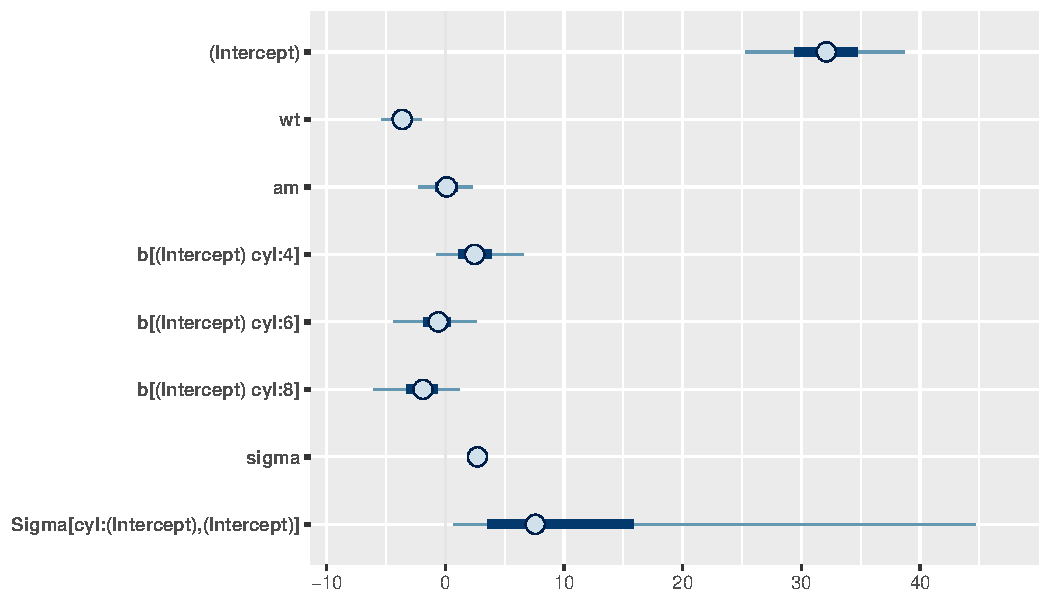
\includegraphics[width=\maxwidth]{figure/p1b-1} \caption[Correlation of given predictors]{Correlation of given predictors.}\label{fig:p1b}
\end{figure}


\end{knitrout}

\end{frame}

%%%%%%%%%%%%%%%%%%%%%%%%%%%%%%%%%%%%%%%%%%%%%%%%%%%%%%%%%%%%%%%%%

\begin{frame}[fragile]
\frametitle{Plot the Results' }



\begin{knitrout}
\definecolor{shadecolor}{rgb}{0.969, 0.969, 0.969}\color{fgcolor}\begin{kframe}
\begin{alltt}
\hlkwd{plot}\hlstd{(brm_re)}
\end{alltt}
\end{kframe}\begin{figure}[H]
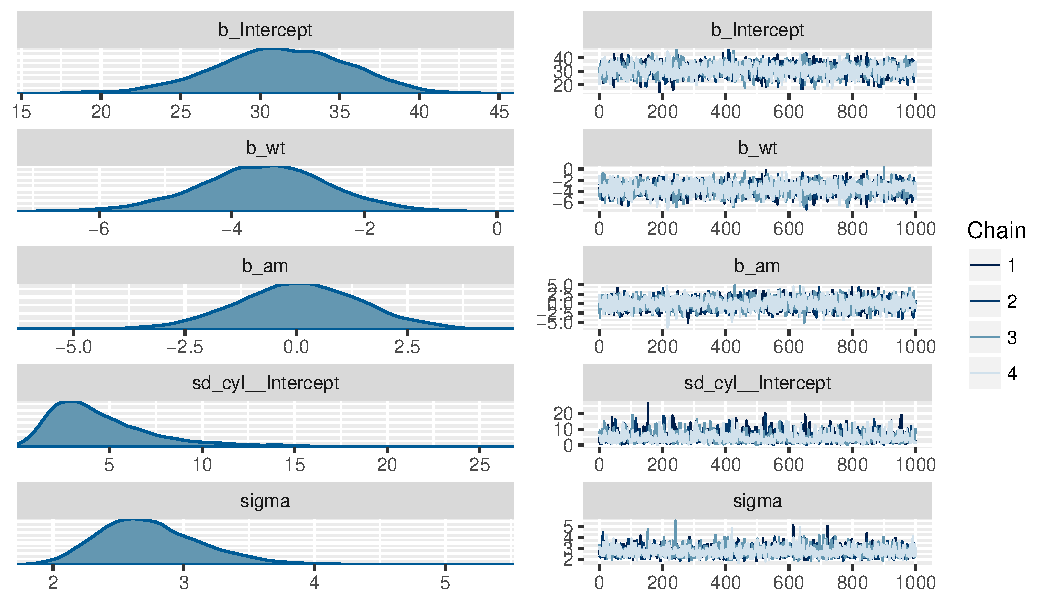
\includegraphics[width=\maxwidth]{figure/p2b-1} \caption[Correlation of given predictors]{Correlation of given predictors.}\label{fig:p2b}
\end{figure}


\end{knitrout}

\end{frame}

%%%%%%%%%%%%%%%%%%%%%%%%%%%%%%%%%%%%%%%%%%%%%%%%%%%%%%%%%%%%%%%%%

\begin{frame}[fragile]
\frametitle{Results' Diagnostics: \texttt{shinystan}}
\texttt{shinystan} workd both for \texttt{stanreg} and \texttt{brmsfit} objects:\\

\begin{knitrout}
\definecolor{shadecolor}{rgb}{0.969, 0.969, 0.969}\color{fgcolor}\begin{kframe}
\begin{alltt}
\hlstd{m1} \hlkwb{<-} \hlkwd{stan_glmer}\hlstd{(}\hlkwc{formula} \hlstd{= mpg} \hlopt{~} \hlstd{wt} \hlopt{+} \hlstd{am} \hlopt{+} \hlstd{(}\hlnum{1}\hlopt{|}\hlstd{cyl),}
                 \hlkwc{data} \hlstd{= mtcars,}  \hlkwc{prior} \hlstd{=} \hlkwa{NULL}\hlstd{,}
                 \hlkwc{family} \hlstd{=} \hlkwd{gaussian}\hlstd{())}

\hlkwd{launch_shinystan}\hlstd{(m1)}
\end{alltt}
\end{kframe}
\end{knitrout}

\end{frame}

%%%%%%%%%%%%%%%%%%%%%%%%%%%%%%%%%%%%%%%%%%%%%%%%%%%%%%%%%%%%%%%%%
\begin{frame}[fragile]
\frametitle{Get the STAN code}
\pause
\texttt{rstanarm: shinystan} \\
\pause
\texttt{brms: make_stancode}!
\begin{knitrout}
\definecolor{shadecolor}{rgb}{0.969, 0.969, 0.969}\color{fgcolor}\begin{kframe}
\begin{alltt}
\hlkwd{make_stancode}\hlstd{(mpg} \hlopt{~} \hlstd{wt} \hlopt{+} \hlstd{am} \hlopt{+} \hlstd{cyl,} \hlkwc{data} \hlstd{= mtcars,}
    \hlkwc{prior} \hlstd{=} \hlkwa{NULL}\hlstd{,} \hlkwc{family}  \hlstd{=} \hlstr{"gaussian"}\hlstd{)}
\end{alltt}
\end{kframe}
\end{knitrout}

model {                                                   \\
  vector[N] mu = Xc * b; \\
  for (n in 1:N) { \\
    mu[n] = mu[n] + (r_1_1[J_1[n]]) * Z_1_1[n];  \\
  } \\
  // priors including all constants \\
  target += student_t_lpdf(temp_Intercept | 3, 0, 10); \\
  target += student_t_lpdf(sd_1 | 3, 0, 10)\\

\end{frame}

%%%%%%%%%%%%%%%%%%%%%%%%%%%%%%%%%%%%%%%%%%%%%%%%%%%%%%%% 

\begin{frame}[fragile]
\frametitle{Some Differences}
\pause
With \texttt{brms} you can also implement multinomial logistic regressions
\begin{knitrout}
\definecolor{shadecolor}{rgb}{0.969, 0.969, 0.969}\color{fgcolor}\begin{kframe}
\begin{alltt}
\hlkwd{brm}\hlstd{(Species} \hlopt{~} \hlstd{Petal.Length} \hlopt{+} \hlstd{Petal.Width} \hlopt{+} \hlstd{Sepal.Length} \hlopt{+}
      \hlstd{Sepal.Width,} \hlkwc{data}\hlstd{=iris,} \hlkwc{family}\hlstd{=}\hlstr{"categorical"}\hlstd{,}
    \hlkwc{prior}\hlstd{=}\hlkwd{c}\hlstd{(}\hlkwd{set_prior}\hlstd{(}\hlstr{"normal (0, 8)"}\hlstd{)))}
\end{alltt}
\end{kframe}
\end{knitrout}


\end{frame}


%%%%%%%%%%%%%%%%%%%%%%%%%%%%%%%%%%%%%%%%%%%%%%%%%%%%%%%%%%%%%%%%%

\begin{frame}[fragile]
\frametitle{Correlations}
With \texttt{brms} you can also deal easily with different correlation structures by specifieng: \\
\begin{itemize}
\item \textbf{cor_arma}: autoregressive-moving average (ARMA) structure. \\
\item \textbf{cor_arr}: response autoregressive (ARR) structure \\
\item \textbf{cor_car}: Spatial conditional autoregressive (CAR) structure \\
\item \textbf{cor_sar}: Spatial simultaneous autoregressive (SAR) structure \\
\item \textbf{cor_bsts}: Bayesian structural time series (BSTS) structure \\
\item \textbf{cor_fixed}: fixed user-defined covariance structure \\
\end{itemize}

\begin{knitrout}
\definecolor{shadecolor}{rgb}{0.969, 0.969, 0.969}\color{fgcolor}\begin{kframe}
\begin{alltt}
\hlkwd{brm}\hlstd{(mpg} \hlopt{~} \hlstd{wt} \hlopt{+} \hlstd{am} \hlopt{+} \hlstd{(}\hlnum{1}\hlopt{|}\hlstd{cyl),} \hlkwc{data} \hlstd{= mtcars,} \hlkwc{prior} \hlstd{=} \hlkwa{NULL}\hlstd{,}
    \hlkwc{family}\hlstd{=}\hlstr{"gaussian"}\hlstd{,} \hlkwd{cor_arma}\hlstd{(}\hlkwc{formula} \hlstd{=} \hlopt{~}\hlnum{1}\hlstd{,} \hlkwc{q} \hlstd{=} \hlnum{1}\hlstd{))}
\end{alltt}
\end{kframe}
\end{knitrout}

\end{frame}

%%%%%%%%%%%%%%%%%%%%%%%%%%%%%%%%%%%%%%%%%%%%%%%%%%%%%%%% 

\begin{frame}
\frametitle{Conclusions}
\pause
\begin{itemize}
\item \texttt{rstanarm} can be the easiest package to start with since precompiled, but it might be limiting (intentionally) for more advanced needs.
\pause
\item \texttt{brms} is more flexible and customizable.
\pause
\item \texttt{rstan} fully flexible, but you need to learn STAN programming (maybe with the help of \texttt{make_stancode}).
\end{itemize}
\end{frame}


%%%%%%%%%%%%%%%%%%%%%%%%%%%%%%%%%%%%%%%%%%%%%%%%%%%%%%%% 

\begin{frame}
\frametitle{\texttt{\# stanarm}}
\pause
\begin{figure}

\includegraphics[scale=0.4]{Twitter4.png}
\end{figure}
\pause
\begin{figure}

\includegraphics[scale=0.4]{Twitter5.png}
\end{figure}
\pause
\begin{figure}
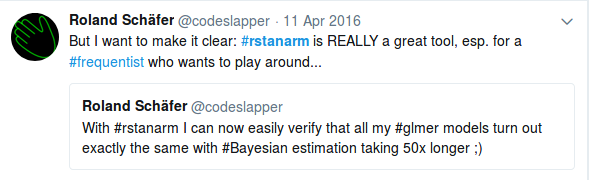
\includegraphics[scale=0.4]{Twitter6.png}
\end{figure}
\end{frame}

%%%%%%%%%%%%%%%%%%%%%%%%%%%%%%%%%%%%%%%%%%%%%%%%%%%%%%%% 

\begin{frame}
\frametitle{\texttt{\# brms}}
\pause
\begin{figure}
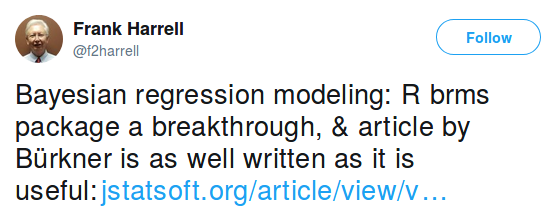
\includegraphics[scale=0.3]{Twitter1.png}
\end{figure}
\pause
\begin{figure}

\includegraphics[scale=0.4]{Twitter2.png}
\end{figure}
\pause
\begin{figure}

\includegraphics[scale=0.4]{Twitter3.png}
\end{figure}
\end{frame}

%%%%%%%%%%%%%%%%%%%%%%%%%%%%%%%%%%%%%%%%%%%%%%%%%%%%%%%%%%

\begin{frame}
\frametitle{Should I be Bayesian?}
\pause
Sampling can be slow \\
\pause
You need to be really careful about diagnostics \\
\pause
You need to have ideas about priors\\
\pause
\textbf{BUT!}\\
\pause
It can help when dealing with small data \\
\pause 
In forecasts since:\\
\textit{"...in terms of forecasting ability, ...a good Bayesian will beat a non-Bayesian, who will do better than a bad Bayesian."} \\
[C.W.J. Granger (1986, p. 16)]\\
\pause
At the end it is a real philosophical question about how you intend statistics. \\

\end{frame}
%%%%%%%%%%%%%%%%%%%%%%%%%%%%%%%%%%%%%%%%%%%%%%%%%%%%%%%%%%

\begin{frame}
\frametitle{The End}

\begin{figure}
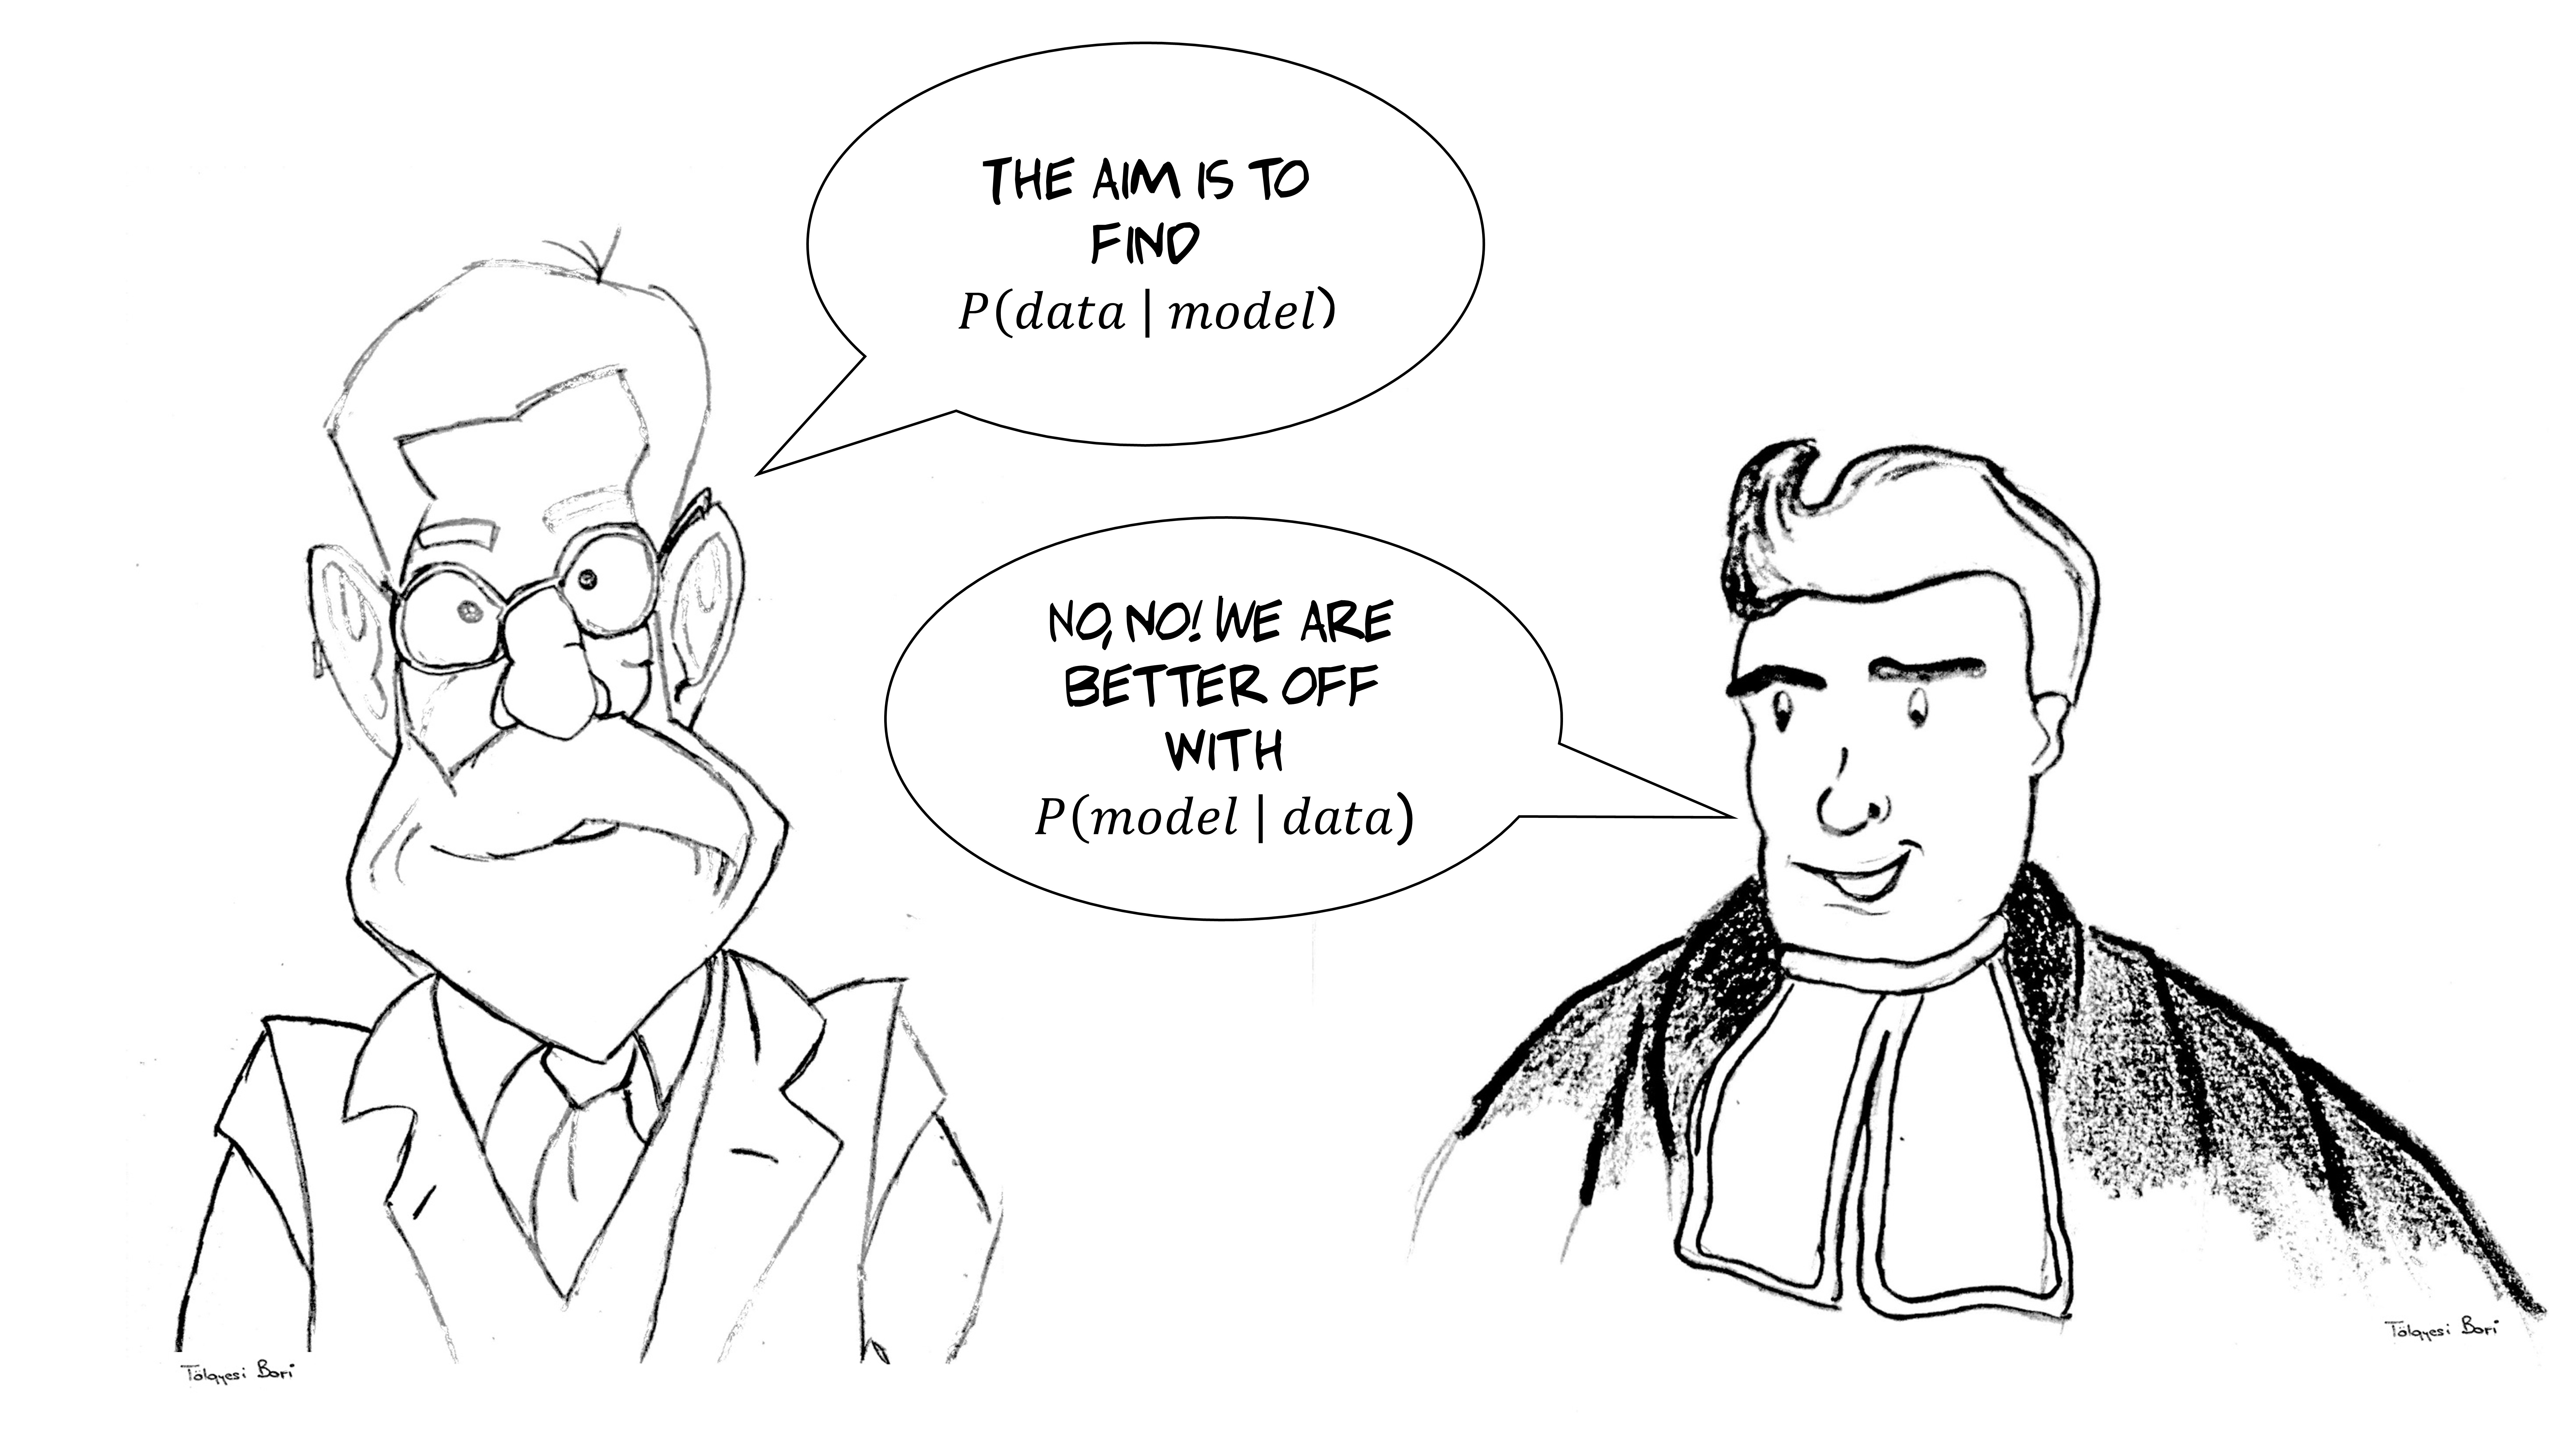
\includegraphics[scale=0.4]{pic1.JPG}
\end{figure}

\end{frame}

%%%%%%%%%%%%%%%%%%%%%%%%%%%%%%%%%%%%%%%%%%%%%%%%%%%%%%%% 
\begin{frame}[allowframebreaks]
\frametitle{References}
\printbibliography

\end{frame}



\end{document}
